\documentclass{article}
\usepackage[T1]{fontenc}
\usepackage[utf8]{inputenc}
\usepackage[polish]{babel}
\usepackage{amsmath}
\usepackage{url}
\usepackage{amssymb}
\usepackage{graphicx}
\usepackage{float}
%{Informatyka stosowana 2020, I st., semestr VI}


\author{
	{Bartosz Kołaciński, 251554}\\
	{Jakub Rosiak, 251620}\\ 
	{Prowadzący: dr. inż. Marcin Kacprowicz}
}

\title{Komputerowe systemy rozpoznawania 2024/2025\\Projekt 1. Klasyfikacja dokumentów tekstowych}
\begin{document}
	\maketitle
	
	\section{Cel projektu}	
	Celem niniejszego projektu jest implementacja, analiza oraz optymalizacja algorytmu k-najbliższych sąsiadów  przeznaczonego do kategoryzacji dokumentów tekstowych na podstawie wyekstrahowanych cech o charakterze liczbowym i tekstowym.
	Klasyfikacja prowadzona jest na zbiorze \textit{Reuters-21578} \cite{reuters21578}, a zadanie polega na przyporządkowaniu artykułów do jednej z 6 klas reprezentujących kraje (USA, UK, Francja, Kanada, Japonia, Niemcy Zachodnie).
	Model uwzględnia zjawisko braku zbalansowania danych (znaczna przewaga artykułów z USA) poprzez zbalansowany podział zbioru na część treningową oraz testową (w proporcji 80/20) i obejmuje zbadanie skuteczności za pomocą metryk Accuracy oraz F1.
	
	\section{Klasyfikacja nadzorowana metodą $k$-NN.  Ekstrakcja cech, wektory cech}
	
	\subsection{Opis metody k-NN w zadaniu kategoryzacji dokumentów}
	Algorytm k-najbliższych sąsiadów (k-NN) to nadzorowana metoda klasyfikacji z grupy metod minimalnoodległościowych \cite{tadeusiewicz90}, polegająca na przypisaniu nowego obiektu do klasy, która najczęściej występuje wśród jego k najbliższych obiektów ze zbioru uczącego (treningowego). W tym zadaniu, każdy dokument jest przekształcany w wielowymiarowy wektor wyekstrahowanych cech.
	Odległość pomiędzy wektorami (dokumentami) obliczana jest na podstawie zdefiniowanej metryki (Euklidesowej dla cech liczbowych i 0/1 dla cech tekstowych). Algorytm przyjmuje jako parametry wejściowe zbiór tekstów, zestaw wag dla każdej z cech oraz liczbę k, a na wyjściu zwraca najbardziej prawdopodobną klasę docelową (kraj, do którego przypisany jest tekst).
	
	\subsection{Ekstrakcja i opis cech wektora}
	Dokumenty reprezentowane są za pomocą zbioru zdefiniowanych cech tekstowych i liczbowych, wyekstrahowanych osobno dla każdego danego artykułu. Niech \(D = (d_1, d_2, ..., d_L)\) oznacza zbiór znaków występujących w artykule o długości \(L\), a \(W = (w_1, w_2, ..., w_N)\) to zbiór \(N\) słów w danym artykule (wyekstrahowanych za pomocą wyrażeń regularnych). Wprowadźmy funkcję pomocniczą \(h(c)\), która przyjmuje wartość 1, gdy warunek \(c\) jest spełniony, oraz 0 w przeciwnym wypadku.
	
	\noindent
	\textbf{Cechy liczbowe:}
	
	1. \textbf{CharCountSpec (\(c_1\)):} Ilość wszystkich znaków w dokumencie bez spacji.
	\begin{equation}
		c_1 = \sum_{j=1}^{L} h(d_j \neq \text{' '})
	\end{equation}
	Zakres wartości: \(\mathbb{N}\)
	
	2. \textbf{WordCountSpec (\(c_2\)):} Ilość wszystkich słów w danym tekście. Słowo jest zdefiniowane jako zbiór znaków oddzielonych spacją.
	\begin{equation}
		c_2 = N = \sum_{j=1}^{N} 1
	\end{equation}
	Zakres wartości: \(\mathbb{N}\).
	
	3. \textbf{AverageWordLengthSpec (\(c_3\)):} Średnia długość słowa.
	\begin{equation}
		c_3 = \frac{1}{N} \sum_{j=1}^{N} |w_j|
	\end{equation}
	Zakres wartości: \(\mathbb{R}_{+} \cup 0\). (Gdy brak słów, cecha równa 0).
	
	4. \textbf{LexicalDiversitySpec (\(c_4\)):} Stosunek ilości unikalnych słów do wszystkich słów w dokumencie. Im większy wynik, tym większy zasób słownictwa w danym tekście. Unikalne słowa badane są bez względu na wielkość znaków. Niech \(U\) będzie zbiorem unikalnych słów z \(W\) zredukowanych do małych liter.
	\begin{equation}
		c_4 = \frac{|U|}{N}
	\end{equation}
	Zakres wartości: \([0, 1]\).
	
	5. \textbf{LongWordToOtherWordsRatioSpec (\(c_5\)):} Stosunek liczby słów długich (co najmniej 5 liter) do liczby pozostałych słów. Niech \(L_w = \sum_{j=1}^{N} h(|w_j|\ge 5)\).
	\begin{equation}
		c_5 = \begin{cases}
			\frac{L_w}{N - L_w} & \text{dla } N - L_w > 0 \\
			L_w & \text{dla } N - L_w <= 0
		\end{cases}
	\end{equation}
	Zakres wartości: \(\mathbb{R}_{+} \cup 0\).
	
	6. \textbf{ProperNounRatioSpec (\(c_6\)):} Współczynnik nazewnictwa własnego – stosunek wyrazów rozpoczynających się wielką literą (z pominięciem tych po znaku końca zdania) do całkowitej ilości słów. 
	Niech \(P = \sum_{j=1}^{N} h(w_j)\) jest nazwą własną\()\).
	\begin{equation}
		c_6 = \frac{P}{N}
	\end{equation}
	Zakres wartości: \([0, 1]\).
	
	7. \textbf{UpperToAllCharsRatioSpec (\(c_7\)):} Stosunek wielkich liter do całkowitej długości tekstu.
	\begin{equation}
		c_7 = \frac{1}{L} \sum_{i=1}^{L} h(d_i \in \text{Wielkie Litery})
	\end{equation}
	Zakres wartości: \([0, 1]\).
	
	8. \textbf{UpperToLowerRatioSpec (\(c_8\)):} Stosunek ilości wielkich liter do małych liter.
	Niech \(U_c = \sum_{i=1}^{L} h(d_i \in \text{Wielkie Litery}\) oraz \(M_c = \sum_{i=1}^{L} h(d_i \in \text{Małe Litery})\)
	\begin{equation}
		c_8 = \begin{cases}
			\frac{U_c}{M_c} & \text{dla } M_c > 0 \\
			U_c & \text{w p. p.}
		\end{cases}
	\end{equation}
	Zakres wartości: \(\mathbb{R}_{+} \cup 0\).
	
	9. \textbf{AlnumToOtherCharsRatioSpec (\(c_9\)):} Stosunek liczby znaków alfanumerycznych (litery i cyfry) do liczby pozostałych znaków (interpunkcja, znaki białe, znaki specjalne).
	Niech \(A_c = \sum_{i=1}^{L} h(d_i \in Alfanumeryczne)\).
	\begin{equation}
		c_9 = \begin{cases}
			\frac{A_c}{L - A_c} & \text{dla } L - A_c > 0 \\
			A_c & \text{dla } L - A_c <= 0
		\end{cases}
	\end{equation}
	Zakres wartości: \(\mathbb{R}_{+} \cup 0\).
	
	\textbf{Cechy tekstowe:}
	
	10. \textbf{ProperNounSpec (\(t_1\)):} Pierwszą napotkana w tekście nazwa własna (wyraz zaczynający się wielką literą, niebędący częścią zdania). Jeśli takiej nie ma, przyjmuje wartość tekstową "None".
	\begin{equation}
		t_1 = w_{j}, \quad \text{gdzie } j = \min \{ i : h(w_i \text{ jest nazwą własną}) = 1 \}
	\end{equation}
	\textit{Przyjmuje wartość "None" jeśli w tekście nie ma nazw własnych}
	Zakres wartości: Ciąg znaków (String).
	
	11. \textbf{RarestRepeatedWordSpec (\(t_2\)):} Wyraz o najmniejszej ilości powtórzeń, jednak pojawiający się przynajmniej dwukrotnie w artykule (redukcja do małych liter). W przypadku remisów wybierane jest słowo pierwsze po sortowaniu alfabetycznie. Jeśli takiego wyrazu nie ma, przyjmuje wartość tekstową "None".
	Niech \(C(w)\) to liczba wystąpień słowa \(u \in U\) w tekście, a \(S = \{u \in U : C(u) \ge 2\}\) zbiór słów powtarzających się.
	\begin{equation}
		t_2 = u \in S : C(u) = \min_{v \in S} C(v)
	\end{equation}
	Zakres wartości: Ciąg znaków (String).
	
	\textbf{Postać wektora cech:}
	
	Na podstawie zaprezentowanych specyfikacji każdy tekst zostaje przekształcony na wektor \(V\) postaci:
	\begin{equation}
		V = [c_1, c_2, c_3, c_4, c_5, c_6, c_7, c_8, c_9, t_1, t_2]
	\end{equation}
	Przykład wektora dla zdania ,,ALFA alfa 123 !!! kot kot Dom dom DOM'':
	\begin{equation}
		V_{przyklad} = [30.0, 8.0, 3.25, 0.5, 0.0, 0.0, 0.25, 0.6, 1.4, \text{''ALFA''}, \text{''alfa''}]
	\end{equation}
	
	\section{Miary jakości klasyfikacji} 
	W celu oceny skuteczności algorytmu \(k\)-NN zastosowano zestaw miar jakości klasyfikacji pozwalających ocenę w skali wszystkich klas, jak i dla pojedynczych krajów. Kluczowe jest rozróżnienie między ogólną dokładnością algorytmu a jego umiejętnością w poprawnym rozpoznawaniu klas rzadkich \cite{tadeusiewicz90}.
	
	\subsection{Parametry i oznaczenia}
	Dla każdej z klas (krajów) \(i \in \{ \text{west-germany, usa, france, uk, canada, japan}\}\) definiujemy następujące parametry:
	\begin{itemize}
		\item \(TP_i\) - liczba dokumentów poprawnie przypisanych do klasy \(i\).
		\item \(actual_i\) - całkowita liczba dokumentów faktycznie należących do klasy \(i\) w zbiorze testowym.
		\item \(predicted_i\) - całkowita liczba dokumentów, które algorytm zaklasyfikował do klasy \(i\).
	\end{itemize}
	
	\subsection{Miary cząstkowe per klasa}
	Dla każdej klasy obliczane są trzy miary, które przyjmują wartości z zakresu $[0, 1]$, gdzie 1 oznacza wynik idealny:
	\begin{enumerate}
		\item \textbf{Precision $P_i$}: Określa, jakie jest prawdopodobieństwo, że dokument zaklasyfikowany do danego kraju faktycznie z niego pochodzi.
		\begin{equation}
			P_i =
			\begin{cases} 
				\frac{TP_i}{Predicted_i} & \text{dla } Predicted_i > 0 \\
				0 & \text{w p.p.} 
			\end{cases}
		\end{equation}
		\item \textbf{Recall $R_i$}: Określa, jaką część wszystkich artykułów z danego kraju udało się poprawnie wykryć algorytmowi.
		\begin{equation}
			R_i =
			\begin{cases}
				\frac{TP_i}{Actual_i} & \text{dla } Actual_i > 0 \\
				0 & \text{w p.p.}
			\end{cases}
		\end{equation}
		\item \textbf{F1-score ($F1_i$)}: Średnia harmoniczna precyzji i pełności..
		\begin{equation}
			F1_i =
			\begin{cases}
				\frac{2 \cdot P_i \cdot R_i}{P_i + R_i} & \text{dla } P_i + R_i > 0 \\
				0 & \text{w p.p.}
			\end{cases}
		\end{equation}
	\end{enumerate}
	
	\subsection{Miary globalne}
	Do globalnej oceny modelu zastosowano:
	\begin{enumerate}
		\item \textbf{Accuracy}: Stosunek wszystkich poprawnych klasyfikacji do liczby wszystkich dokumentów \(M\).
		\begin{equation}
			Acc = \frac{\sum_{i=1}^{6} TP_i}{M}
		\end{equation}
		\item \textbf{Macro-F1}: Średnia arytmetyczna wartości F1 dla wszystkich klas.
		\begin{equation}
			MacroF1 = \frac{1}{6} \sum_{i=1}^{6} F1_i
		\end{equation}
	\end{enumerate}
	
	\subsection{Wyniki i ich interpretacja}
	Przykładowe wartości z przeprowadzonego testu (\(k = 5\) oraz stosunek danych treningowych do testowych \(80 : 20\)):\\
	\begin{table}[h!]
		\centering
		\begin{tabular}{|l|c|c|c|}
			\hline
			\textbf{Klasa (kraj)} & \textbf{Precision (\(P_i\))} & \textbf{Recall (\(R_i\))} & \textbf{F1-score (\(F1_i\))} \\ \hline
			usa & 82,75\%  & 94,81\% & 88,37\% \\ \hline
			canada & 53,06\% & 15,29\% & 23,74\% \\ \hline 
			japan & 34,38\% & 22,00\% & 26,83\% \\ \hline \hline
			
			\textbf{Miara globalna} & \multicolumn{2}{c|}{\textbf{Nazwa}} & \textbf{Wartość} \\ \hline
			Accuracy (Acc) & \multicolumn{2}{c|}{Ogólna dokładność modelu} & \textbf{78,91\%} \\ \hline
			Macro-F1 & \multicolumn{2}{c|}{Średnia harmoniczna klas} & \textbf{34,55\%} \\ \hline
		\end{tabular}
		\caption{Zestawienie przykładowych miar jakości klasyfikacji dla $k=5$.}
	\end{table}
	
	\noindent
	Algorytm osiągnął dokładność bliską \(79\%\), jednak łatwo zauważyć niskie wartości miar dla krajów innych niż USA, wynika to z znacznej przewagi USA w danych. Macro-F1 znacznie lepiej odzwierciedla słabości modelu (jego niską stabilność) w rozpoznawaniu innych klas.
	
	\newpage
	\section{Metryki i miary podobieństwa tekstów w klasyfikacji}
	
	Ważną częścią metody \(k\)-NN jest wybór metryk i miar do obliczania odległości między dwoma danymi wektorami cech. Aby zapobiec dominacji cech, które mogą przyjmować duże wartości (np. liczba znaków w danym tekście) stosujemy normalizacje min-max do przedziału \([0;1]\) na podstawie granicznych wartości znajdujących się w zbiorze testowym. Niech \(n\) będzie oznaczeniem funkcji wykorzystanej do normalizacji.
	
	Niech \(V^a\) i \(V^b\) będą dwoma wektorami cech, a \(w_i\) wagą przypisaną do \(i\)-tej cechy. Dla cech liczbowych odległość dla \(i\)-tej cechy liczbowej określamy następująco:
	\begin{equation}
		\delta_i(V^a, V^b) = |n(V^a_i) - n(V^b_i)|
	\end{equation} 
	
	\noindent
	Dla \(i\)-tej cechy tekstowej wartość składowej odległości obliczamy za pomocą:
	\begin{equation}
		\delta_i(V^a, V^b) = d_J(V^a_i, V^b_i)
	\end{equation}
	gdzie \(d_J\) to odległość Jaccarda oparta na \(n\)-gramach.
	
	\subsection{Miara podobieństwa tekstów - n-gramy}
	W celu obliczenia odległości między cechami tekstowymi zastosowano metodę bazującą na zbiorach \(n\)-gramów dla \(n=2\). Niech \(s\) będzie dowolnym ciągiem znaków, a \(G_n(s)\) to zbiór wszystkich podciągów o długości \(n\) z tekstu \(s\). Dla \(s=\texttt{'ALFA'}\): \(G_2(\texttt{'ALFA'}) = \{\texttt{'AL', 'LF', 'FA'}\}\).
	
	Podobieństwo Jaccarda (\(J\)) dwóch tekstów (\(t_a\) i \(t_b\)) definiujemy jako stosunek mocy części wspólnej zbiorów ich bigramów do mocy ich sumy:
	\begin{equation}
		J(t_a, t_b) = \frac{|G_2(t_a) \cap G_2(t_b)|}{|G_2(t_a) \cup G_2(t_b)|}
	\end{equation}
	
	Ostateczna miara odległości jest opisana za pomocą wzoru:
	\begin{equation}
		d_J(t_a, t_b) = 1 - J(t_a, t_b)
	\end{equation}
	Dla dwóch identycznych tekstów \(t_a\) i \(t_b\) \(J(t_a,t_b)\) przyjmuje wartość 1, więc odległość wynosi 1.
	
	\subsection{Zastosowane metryki}
	Na podstawie obliczonych odległości \(\delta_i\) oraz wag \(w_i\), odległość całkowitą \(D(V^a,V^b)\) oblicza się przy użyciu jednej z metryk:
	
	\subsubsection{Metryka Euklidesowa}
	\begin{equation}
		D(V^a,V^b) = \sqrt{\sum_{i=1}^{i=11} (w_i \cdot \delta_i)^2}
	\end{equation}
	
	\subsubsection{Metryka Manhattan (uliczna)}
	\begin{equation}
		D(V^a,V^b) = \sum_{i=1}^{i=11} w_i \cdot \delta_i
	\end{equation}
	
	\subsubsection{Metryka Czebyszewa}
	\begin{equation}
		D(V^a,V^b) = \max_{i} (w_i \cdot \delta_i)
	\end{equation}
	
	\subsection{Obliczanie przykładowych wartości}
	Rozważmy dwa proste wektory cech \(V^1\) i \(V^2\) (z cechami \(c_1, c_2, c_3\)) z wagami równymi \(1\):
	\begin{itemize}
		\item \(V^1 = [0.6, 0.7, \texttt{'LONDON'}]\)
		\item \(V^2 = [0.4, 0.8, \texttt{'LONDONER'}]\)
	\end{itemize}
	
	\noindent
	Obliczenia składowe:
	\begin{itemize}
		\item \(\delta_1 = |0.6 - 0.4| = 0.2\)
		\item \(\delta_2 = |0.7 - 0.8| = 0.1\)
		\item \(G(c_3^1) = \{LO, ON, ND, DO, ON\}\) \(\rightarrow\) \(\{LO, ON, ND, DO\}\)
		\item \(G(c_3^2) = \{LO, ON, ND, DO, ON, NE, ER\}\) \(\rightarrow\) \(\{LO, ON, ND, DO, NE, ER\}\)
		\item \(J = \frac{|\{LO, ON, ND, DO\}|}{|\{LO, ON, ND, DO, NE, ER\}|} = \frac{2}{3} \approx 0.67\)
		\item \(\delta_3 = 1 - 0.67 = 0.33\)
	\end{itemize}
	
	\noindent
	Wyniki dla różnych metryk:
	\begin{itemize}
		\item \(D_{euklides} = \sqrt{0.2^2 + 0.1^2 + 0.33^2} \approx 0.4\)
		\item \(D_{manhattan} = 0.2 + 0.1 + 0.33 = 0.53\)
		\item \(D_{czebyszew} = \max(0.1, 0.2, 0.33) = 0.33\)
	\end{itemize}
	
	\newpage
\section{Wyniki klasyfikacji dla różnych parametrów wejściowych}

W niniejszej sekcji przedstawiono wstępne wyniki miary \textbf{Accuracy} dla próbnych klasyfikacji na ograniczonym zbiorze tekstów. Eksperymenty przeprowadzono zgodnie z założeniami projektu (punkty 3--8), obejmującymi dobór parametrów modelu, metryk odległości oraz podział danych.

\subsection{Eksperyment 1: Wpływ parametru $k$ oraz metryki odległości na Accuracy}

W pierwszym eksperymencie analizowano wpływ liczby sąsiadów $k$ na jakość klasyfikacji dla trzech metryk odległości:
\begin{itemize}
    \item metryka euklidesowa,
    \item metryka Manhattan,
    \item metryka Czebyszewa.
\end{itemize}

Dla każdej metryki rozpoczęto od wartości $k = 1$, a następnie zwiększano $k$ iteracyjnie. Proces zwiększania parametru $k$ był kontynuowany do momentu, w którym przez trzy kolejne wartości $k$ nie zaobserwowano poprawy wartości Accuracy. Następnie porównano uzyskane wyniki dla poszczególnych metryk.

\begin{figure}[H]
    \centering
    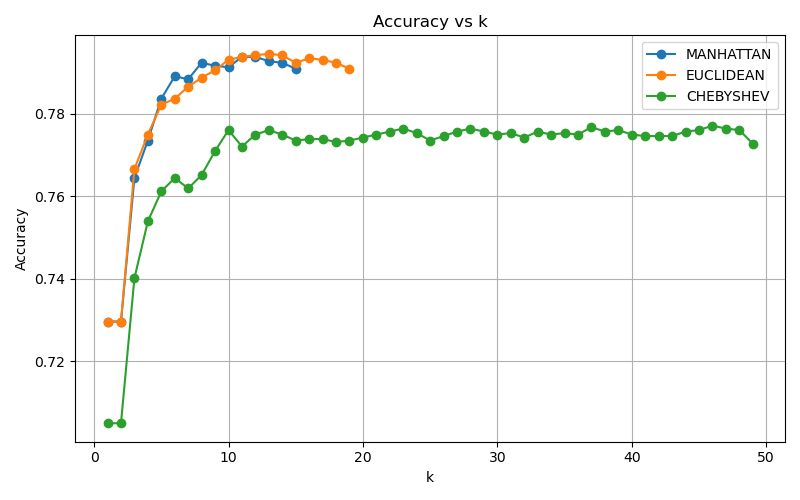
\includegraphics[width=0.8\textwidth]{acc_vs_k.png}
    \caption{Accuracy w funkcji parametru $k$ dla różnych metryk odległości}
    \label{fig:exp1}
\end{figure}

\newpage
Najlepszy wynik uzyskany w eksperymencie 1 wyniósł:
\begin{itemize}
    \item $k = 13$
    \item wielkość zbioru testowego = 20,00\%
    \item metryka = euklidesowa
    \item liczba cech = 11
    \item Accuracy = 0,794555
\end{itemize}

\subsection{Eksperyment 2: Wpływ wielkości zbioru testowego na Accuracy (metryka euklidesowa)}

W drugim eksperymencie badano wpływ procentowego podziału danych na zbiór treningowy i testowy na skuteczność klasyfikacji. Wykorzystano metrykę euklidesową oraz stałą wartość parametru $k = 5$.

Testowano wszystkie proporcje zbioru testowego od 10\% do 90\% ze skokiem co 5\%, tj.:
\begin{itemize}
    \item 10\%, 15\%, 20\%, \dots, 85\%, 90\%.
\end{itemize}

Dla każdej konfiguracji obliczono Accuracy i przeanalizowano stabilność wyników.

\begin{figure}[H]
    \centering
    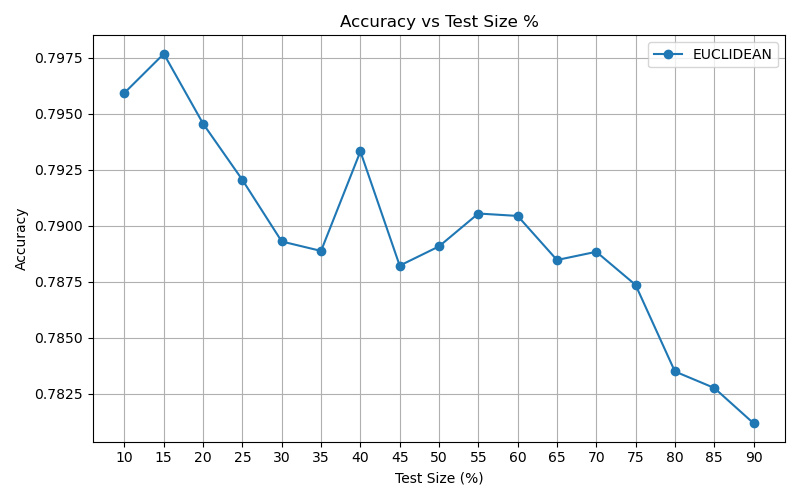
\includegraphics[width=0.8\textwidth]{acc_vs_test_size.png}
    \caption{Wpływ wielkości zbioru testowego na (Accuracy) (metryka euklidesowa)}
    \label{fig:exp2}
\end{figure}

\newpage
Najlepszy wynik w eksperymencie 2 uzyskano dla:
\begin{itemize}
    \item $k = 13$
    \item wielkość zbioru testowego = 20,00\%
    \item metryka = euklidesowa
    \item liczba cech = 11
    \item Accuracy = 0,794555
\end{itemize}

\subsection{Eksperyment 3: Wpływ cech na Accuracy}

W trzecim eksperymencie analizowano wpływ poszczególnych cech (feature'ów) na skuteczność klasyfikacji. Badanie polegało na:
\begin{itemize}
    \item trenowaniu modelu z wykorzystaniem wszystkich cech,
    \item usuwaniu pojedynczych cech i obserwacji zmiany Accuracy.
\end{itemize}

Model trenowano dla $k=13$, przy teście podzielonym na 15\% danych oraz wykorzystaniu metryki EUCLIDEAN. Najlepsze uzyskane Accuracy wyniosło $0,802033$. Poniższa tabela przedstawia zestawy cech, które osiągnęły tę najwyższą wartość Accuracy:

\begin{table}[H]
\centering
\begin{tabular}{|c|}
\hline
\textbf{Zestaw cech} \\ \hline
\begin{tabular}[c]{@{}l@{}}
alnumToOtherCharsRatio, charCount, longWordToOtherWordsRatio, \\
properNounMidSentenceRatio, properNounFirst, rarestRepeatedWord, \\
upperToAllCharsRatio, upperToLowerRatio, wordCount
\end{tabular} \\ \hline
\begin{tabular}[c]{@{}l@{}}
alnumToOtherCharsRatio, charCount, longWordToOtherWordsRatio, \\
properNounFirst, rarestRepeatedWord, upperToAllCharsRatio, \\
upperToLowerRatio, wordCount
\end{tabular} \\ \hline
\begin{tabular}[c]{@{}l@{}}
alnumToOtherCharsRatio, charCount, longWordToOtherWordsRatio, \\
properNounMidSentenceRatio, rarestRepeatedWord, upperToAllCharsRatio, \\
upperToLowerRatio, wordCount
\end{tabular} \\ \hline
\begin{tabular}[c]{@{}l@{}}
alnumToOtherCharsRatio, charCount, longWordToOtherWordsRatio, \\
properNounMidSentenceRatio, properNounFirst, rarestRepeatedWord, \\
upperToLowerRatio, wordCount
\end{tabular} \\ \hline
\begin{tabular}[c]{@{}l@{}}
alnumToOtherCharsRatio, charCount, longWordToOtherWordsRatio, \\
properNounMidSentenceRatio, properNounFirst, rarestRepeatedWord, \\
upperToAllCharsRatio, wordCount
\end{tabular} \\ \hline
\end{tabular}
\caption{Najlepsze zestawy cech w eksperymencie 3 uzyskujące Accuracy = 0,802033}
\label{tab:exp3_best_features}
\end{table}

\begin{figure}[H]
    \centering
    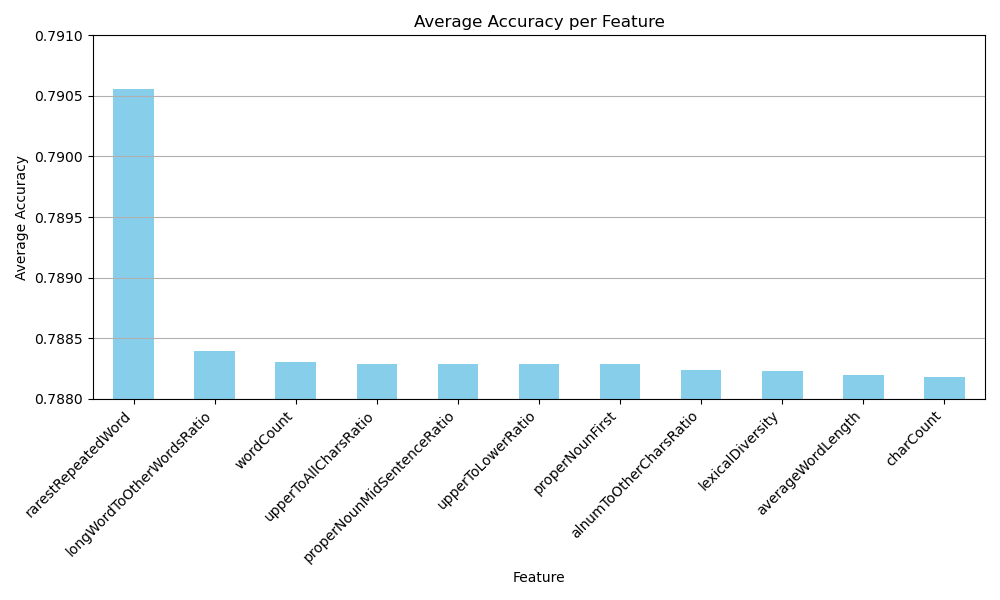
\includegraphics[width=0.9\textwidth]{avg_acc_per_feature.png}
    \caption{Średnie Accuracy uzyskane przy usuwaniu pojedynczych cech. Wykres pokazuje, które cechy mają największy wpływ na jakość klasyfikacji.}
    \label{fig:exp3_feature_impact}
\end{figure}



\newpage
	\section{Dyskusja, wnioski, sprawozdanie końcowe}
	We wnioskach z badania skomentować wyłącznie wpływ parametrów i cech na jakość procesu klasyfikacji. Innymi słowy – wnioski to to, co wynika z przeprowadzonych obliczeń, a nie to co wiadomo z literatury. 
	Znaczenie kolejnych eksperymentów wg punktów 2.-8. opisu projektu 1.  Każdorazowo
	podane parametry, dla których przeprowadzana eksperyment. 
	Wykresy (np. słupkowe) i tabele wyników
	obowiązkowe, dokładnie opisane w ,,captions'' (tytułach), konieczny opis osi i
	jednostek wykresów oraz kolumn i wierszy tabel.\\ 
	
	{**Ewentualne wyniki realizacji punktu 9. opisu Projektu 1., czyli ,,na ocenę 5.0'' i ich porównanie do wyników z
		części obowiązkowej**.Dokładne interpretacje uzyskanych wyników w zależności od parametrów klasyfikacji
		opisanych w punktach 3.-8 opisu Projektu 1. 
		Omówić i wyjaśnić napotkane problemy (jeśli były). Każdy wniosek/problem powinien mieć poparcie
		w przeprowadzonych eksperymentach (odwołania do konkretnych wyników: wykresów,
		tabel). \\
		\underline{Dla końcowej oceny jest to najważniejsza sekcja} sprawozdania, gdyż prezentuje poziom
		zrozumienia rozwiązywanego problemu.\\
		
		** Możliwości kontynuacji prac w obszarze systemów rozpoznawania, zwłaszcza w kontekście pracy inżynierskiej,
		magisterskiej, naukowej, itp. **\\
		
		\noindent {\bf Sekcja uzupełniona jako efekt zadań Tydzień 05 i Tydzień 06 wg Harmonogramu Zajęć
			na WIKAMP KSR.}
		
		
		\section{Braki w realizacji projektu 1.}
		Wymienić wg opisu Projektu 1. wszystkie niezrealizowane obowiązkowe elementy projektu, ewentualnie
		podać merytoryczne (ale nie czasowe) przyczyny tych braków. 
		
		
		\begin{thebibliography}{0}
			\bibitem{tadeusiewicz90} R. Tadeusiewicz: Rozpoznawanie obrazów, PWN, Warszawa, 1991.  
			\bibitem{niewiadomski08} A. Niewiadomski, Methods for the Linguistic Summarization of Data: Applications of Fuzzy Sets and Their Extensions, Akademicka Oficyna Wydawnicza EXIT, Warszawa, 2008.
			\bibitem{reuters21578} David Lewis, \textit{Reuters-21578 Text Categorization Collection}, UCI Machine Learning Repository, 1997. Dostępne online: \url{https://archive.ics.uci.edu/dataset/137/reuters+21578+text+categorization+collection}
		\end{thebibliography}
	\end{document}
